\documentclass[a4paper]{article}
\usepackage[utf8]{inputenc}
\usepackage{graphicx}
\usepackage{multicol}
\usepackage{amsmath}
\usepackage[export]{adjustbox}
\usepackage[bottom=2.0cm,top=2.0cm,left=2.0cm,right=2.0cm]{geometry}
\usepackage[portuges]{babel}
\usepackage{indentfirst}
\usepackage{hyperref} 
\hypersetup{colorlinks,citecolor=black,filecolor=black,linkcolor=black,urlcolor=black}
\bibliographystyle{ieeetr}
\usepackage{float}



\begin{document}
	\title{Template dos relatórios de Métodos da Física Experimental}
	
	
	\begin{titlepage}
		\begin{center}
			\begin{figure}[htb!]
				\begin{flushleft}
					
\includegraphics[width=3.9cm]{latex/1024px-Ufu_logo.svg (2)}
				\end{flushleft}
			\end{figure}
			\vspace{-3,5cm}
			\begin{flushright}
				\Large{\textbf{Universidade Federal de Uberlândia}}\\
			\Large{Faculdade de Engenharia Elétrica}\\
			\Large{Eletromagnetismo (GEE517)}\\
			\end{flushright}
			
			\vspace{200pt}
			
			\LARGE{\textbf{Relatório:}}\\ 
			\Large{Simulação FEMM de um Capacitor Esférico}\\
			
			\vspace{150pt}
			
			
			\vspace{40pt} 
			\hfill Matheus Felipe Lima\hspace{20pt} Matrícula: 41921ETE006
			
			\vspace{25pt}
			\hfill \underline{Professor:}\\
			\hfill Gustavo Nozella Rocha\\
			
			
			\vspace{\fill}
			\LARGE \bf{\today}
			
		\end{center}
	\end{titlepage}
	
	
	\newpage
	
	\pagenumbering{arabic}
	\large
	
	
	\begin{multicols}{2}
	
	\section{Resumo} \label{sec:Resumo}
	
	Potencial elétrico é a capacidade que um corpo energizado tem de realizar trabalho, ou seja, atrair ou repelir outras cargas elétricas. Com relação a um campo elétrico, interessa-nos a capacidade de realizar trabalho, associada ao campo em si, independentemente do valor da carga q colocada num ponto desse campo. Para medir essa capacidade, utiliza-se a grandeza potencial elétrico.\cite{wiki:peletrico}\\
	
	Um campo elétrico é o campo de força provocado pela ação de cargas elétricas, (elétrons, prótons ou íons) ou por sistemas delas. Cargas elétricas colocadas num campo elétrico estão sujeitas à ação de forças elétricas, de atração e repulsão.\cite{wiki:celetrico}\\
	
	A capacitância ou capacidade elétrica é a grandeza escalar que mede a capacidade de armazenamento de energia em equipamentos e dispositivos elétricos, relacionando carga com diferença de potencial.\cite{capacitancia}\\
	
	Deseja-se, através da um paralelo entre a teoria e a simulação, analisar o potencial, campo elétrico e a capacitância entre duas esferas concêntricas de um capacitor.
	
	\section{Objetivo} \label{sec:Objetivo}
	Dado um capacitor com duas esferas concêntricas onde $V(r=0,5[cm])=0 [V]$ e $V(r=2[cm])=20 [V]$ e a região entre as esferas está livre de cargas, será feita uma análise quanto ao potencial, campo elétrico e a capacitância armazenada em três dielétricos: ar, porcelana e sílica fundida.
	
	
	\begin{table} [H]
		\centering
		\caption{Constante dielétrica relativa \cite{wiki:xxx}\label{tab:constantes}}
		\begin{tabular}{|c|c|}
			\hline
			Material & $\epsilon _{r}$ \\
			\hline
			Ar & 1,00059 \\
			\hline
			Porcelana & 6,0 \\
			\hline
			Sílica fundida & 3,8 \\
			\hline
		\end{tabular}
	\end{table}
	
	
	\section{Método}
	Utilizou-se a teoria junto aos cálculos numéricos e os resultados das simulações para discussão.
	\subsection{Teoria}
	Considerando que a densidade volumétrica de cargas é nula entre as esferas, aplica-se a equação de Laplace
	
	\begin{equation} \label{eq:laplaciano}
		\boxed{\bigtriangledown ^2V=\frac{1}{r^2}\frac{\partial }{\partial r}\left(r^2\frac{\partial }{\partial r}\left(V\right)\right)=0}
	\end{equation}
	
	Nota-se que o laplaciano contém apenas o termo da parcial em relação à r, isso porque, devido a simetria do problema, V depende apenas desse parâmetro.\\
	
	Isolando V, chegamos na equação
	
	\begin{equation} \label{eq:potencialab}
		\boxed{V(r)=-\frac{A}{r}+B} 
	\end{equation}
	
	\noindent onde deve-se determinar A e B através do sistema dado os valores introduzidos e compor a equação que determina o potencial elétrico
	
	\begin{equation} \label{eq:matriz}
		\boxed{\left\{\begin{matrix}
		V\left(0,5\cdot 10^{-2}\right)=-\frac{A}{0,5\cdot 10^{-2}}+B=0
		\\ 
		V\left(2\cdot 10^{-2}\right)=-\frac{A}{2\cdot 10^{-2}}+B=20
	\end{matrix}\right.}
	\end{equation}
	
	
	\begin{equation} \label{eq:potencial}
		\boxed{V\left(r[m]\right)=-\frac{2}{15r}+\frac{80}{3}}
	\end{equation}


\begin{figure} [H]
	\centering
	\caption{Potencial[V] $vs$ Raio[m]\label{fig:potencial}}
	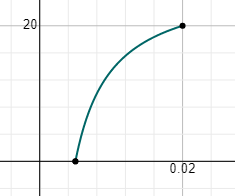
\includegraphics[height=6cm,fbox]{latex/vr.png}
\end{figure}
	
	A partir desta também encontramos a função intensidade do campo elétrico

	\begin{equation} \label{eq:campo}
		\boxed{|\overline{E}|=-\bigtriangledown V=\frac{2}{15r^2}}
	\end{equation}
\\
\begin{figure} [H]
	\centering
	\caption{Campo Elétrico[V/m] $vs$ Raio[m]\label{fig:campo}}
	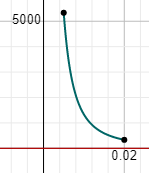
\includegraphics[height=5cm,fbox]{latex/campo.png}
\end{figure}
	
	Para determinar capacitância em um capacitor esférico, dado por
	
	\begin{equation} \label{eq:capacitancia}
		\boxed{C=\frac{4\pi \epsilon }{\:\frac{1}{a}-\frac{1}{b}}}
	\end{equation}
	
	\noindent onde a é o raio da esfera interna e b o da esfera externa, obtemos a seguinte relação para os diferentes tipos de dielétricos
	
	\begin{table} [H]
		\centering
	    \caption{Capacitância\label{tab:capacitancia}}
		\begin{tabular}{|c|c|}
		\hline
		Material & C [F] \\
		\hline
		Ar & $7,412\cdot10^{-13}$ \\
		\hline
		Porcelana & $4,445\cdot10^{-12}$ \\
		\hline
		Sílica fundida & $2,815\cdot10^{-12}$ \\
		\hline
	\end{tabular}
	\end{table}
	
	\subsection{Simulação}
	Utilizou-se o software FEMM para simular as condições dadas. A princípio foi feito a construção da geometria do problema no CAD e dado início a simulação, como mostra a Figura \ref{fig:simulacao}.

	\begin{figure} [H]
		\centering
		\caption{Simulação\label{fig:simulacao}}
		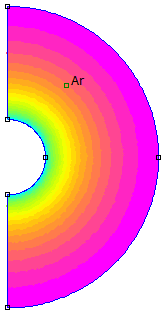
\includegraphics[width=4cm,fbox]{latex/Screenshot_1.png}
	\end{figure}

	A imagem 2D, na verdade, preenche 360 graus em um giro no eixo vertical, formando o capacitor 3D como no problema.\\
	
	Obteve-se também os gráficos mostrados na Figura \ref{fig:potencial_simu} e \ref{fig:campo_simu}
	
	\begin{figure} [H]
		\centering
		\caption{Potencial Elétrico[V] $vs$ Raio[cm]\label{fig:potencial_simu}}
		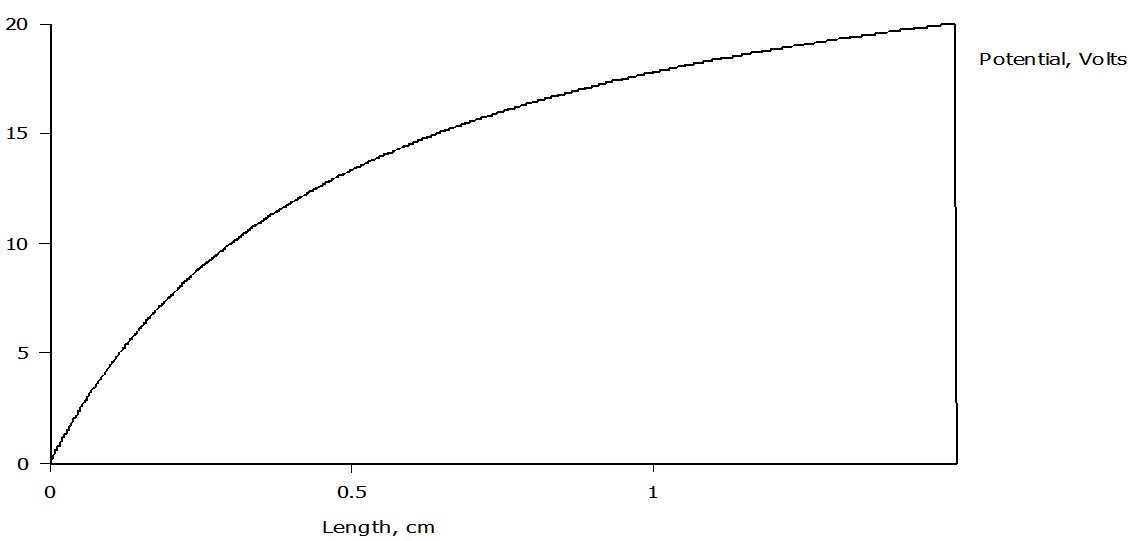
\includegraphics[width=8cm ,fbox]{latex/potencial1.png}
	\end{figure}

\begin{figure} [H]
	\centering
	\caption{Campo Elétrico[V/m] $vs$ Raio[cm]\label{fig:campo_simu}}
	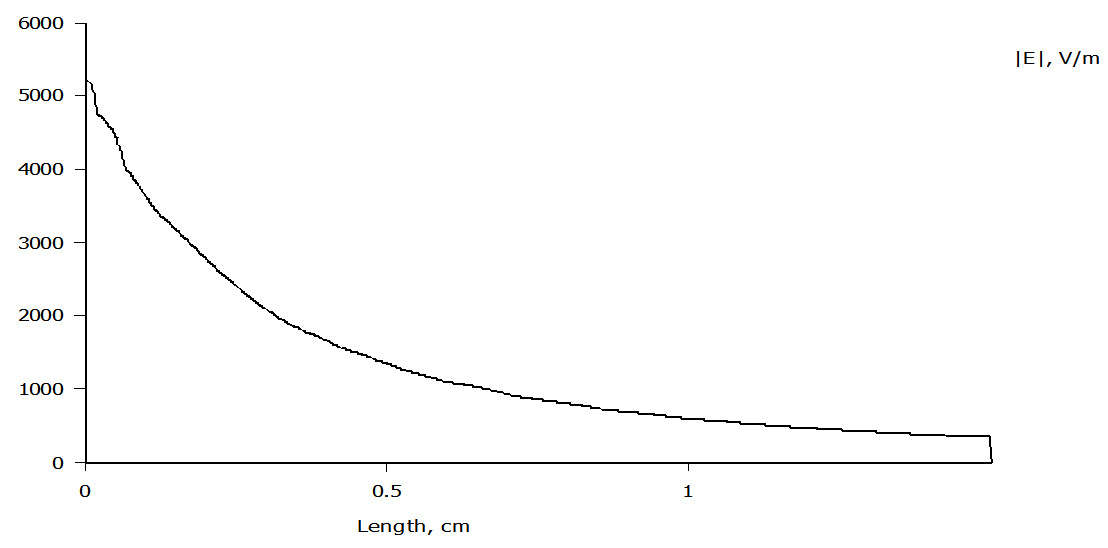
\includegraphics[width=8cm ,fbox]{latex/campo1.png}
\end{figure}
	
	\noindent traçando uma reta horizontal entre as duas extremidades mais próximas, i.e., de r variando de 0,5[cm] até 2[cm].\\
	
	Quanto a capacitância, foi obtido, conforme as Figuras \ref{fig:Qar}, \ref{fig:Qporcelana} e \ref{fig:Qsilica}, a densidade superficial de cargas nos condutores externos para cada material.
	
	\begin{figure} [H]
		\centering
		\caption{Densidade de cargas; Ar\label{fig:Qar}}
		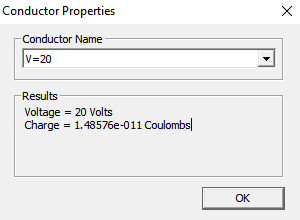
\includegraphics[width=8cm ,fbox]{latex/Qar.png}
	\end{figure}
	
	\begin{figure} [H]
		\centering
		\caption{Densidade de cargas; Porcelana\label{fig:Qporcelana}}
		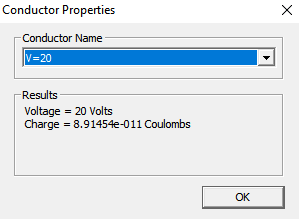
\includegraphics[width=8cm ,fbox]{latex/Qporcelana.png}
	\end{figure}
	
	\begin{figure} [H]
		\centering
		\caption{Densidade de cargas; Sílica Fundida\label{fig:Qsilica}}
		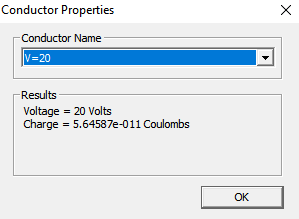
\includegraphics[width=8cm ,fbox]{latex/Qsilica.png}
	\end{figure}

	Chegando na Tabela \ref{tab:capacitancia1} por meio da Equação \ref{eq:capacitancia1}.
	
	\begin{equation} \label{eq:capacitancia1}
		\boxed{C=\frac{Q}{V}}
	\end{equation}

	\begin{table} [H]
		\centering
		\caption{Capacitância\label{tab:capacitancia1}}
		\begin{tabular}{|c|c|}
			\hline
			Material & C [F] \\
			\hline
			Ar & $7,429\cdot10^{-13}$ \\
			\hline
			Porcelana & $4,458\cdot10^{-12}$ \\
			\hline
			Sílica fundida & $2,823\cdot 10^{-12}$ \\
			\hline
		\end{tabular}
	\end{table}
	
	\section{Comparação} \label{sec:comparacao}
	Analisando visualmente os gráficos, percebe-se uma coerência nos resultados obtidos. Para além, convém determinar o erro.\\
	
	Obteve-se 1500 pontos de V e r por meio do FEMM e, utilizando o MatLab, foi feita a subtração do potencial teórico em cada valor de r com o obtido pela simulação; dividido pela quantidade de pontos, conforme a Figura \ref{fig:potencialerro}.
	
	\begin{figure} [H] 
		\centering
		\caption{Erro de V calculado no MatLab\label{fig:potencialerro}}
		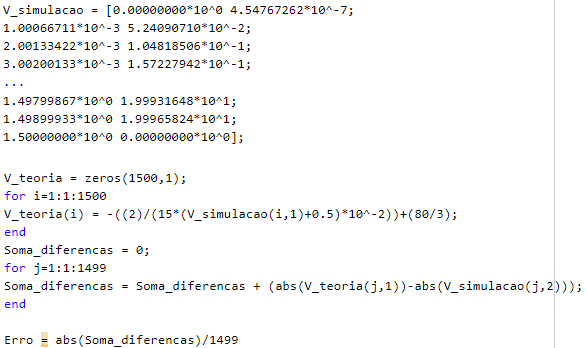
\includegraphics[width=8cm ,fbox]{latex/matlab.png}
	\end{figure}

	Resultando em um erro médio de 0,0071[V]. O último ponto foi desconsiderado pois não obedece a Equação \ref{eq:potencial} já que V é 0 nos pontos da superfície condutora.\\
	
	O mesmo foi realizado para o campo elétrico onde o erro médio encontrado foi de 1,76[V/m].
	
	\begin{figure} [H]
		\centering
		\caption{Erro de $ |E| $ calculado no MatLab}
		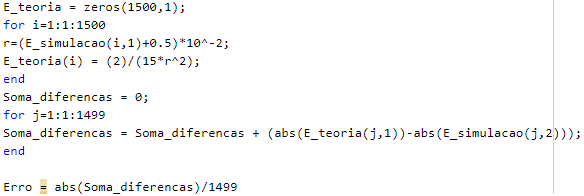
\includegraphics[width=8cm ,fbox]{latex/matlab1.png}
	\end{figure}

	O erro médio da capacitância entre o a simulação e teoria dado os três dielétricos foi de $7,56667\cdot 10^{-15}$[F].
	
	\section{Conclusão}
	Os conceitos e cálculos teóricos puderam se provar com a simulação, entretanto o erro poderia ser amenizado aumentando o número de nós, i.e., de elementos finitos. Percebe-se, conforme a Tabela \ref{tab:capacitancia} e Equação \ref{eq:capacitancia}, que quanto maior o $\epsilon_{r}$, maior a capacitância do capacitor, o que também se provou com a simulação; fazendo com que o ar, muito utilizado em cálculos teóricos, não seja utilizado como dielétrico em capacitores pela sua baixa constante dielétrica. Percebe-se, com os cálculos da Seção \ref{sec:comparacao}, um erro maior para o campo elétrico comparado ao potencial elétrico, o que faz sentido levando em conta o termo ao quadrado no denominador da Equação \ref{eq:campo}.
	
	
	
	\end{multicols}

\newpage
\bibliography{Bibliografia}

\end{document}